\documentclass[ngerman,hyperref={pdfpagelabels=false}]{beamer}

% -----------------------------------------------------------------------------

\graphicspath{{images/}}
\usepackage{graphics}
\usepackage{multimedia}
% -----------------------------------------------------------------------------

\usetheme{KIT}

\setbeamercovered{transparent}
%\setbeamertemplate{enumerate items}[ball]

\newenvironment<>{KITtestblock}[2][]
{\begin{KITcolblock}<#1>{#2}{KITblack15}{KITblack50}}
{\end{KITcolblock}}

\usepackage[ngerman,english]{babel}
\usepackage{animate}
\usepackage[utf8]{inputenc}
\usepackage[TS1,T1]{fontenc}
\usepackage{array}
\usepackage{multicol}
\usepackage[absolute,overlay]{textpos}
\usepackage{beamerKITdefs}
\usepackage[ruled,vlined,linesnumbered,norelsize]{algorithm2e}

\pdfpageattr {/Group << /S /Transparency /I true /CS /DeviceRGB>>}	%required to prevent color shifting withd transparent images


\title{SAT Solving with distributed local search}
\subtitle{Guangping Li -- \textit{uzdif@student.kit.edu}}

\author[Guangping Li]{Guangping Li}
\institute{Institute of Theoretical informatics, Algorithmics II}

\TitleImage[width=\titleimagewd,height=\titleimageht]{titel}

\KITinstitute{Institute of Theoretical informatics}
\KITfaculty{KIT Department of Informatics}

% -----------------------------------------------------------------------------

\begin{document}
\setlength\textheight{7cm} %required for correct vertical alignment, if [t] is not used as documentclass parameter


% title frame
\begin{frame}
  \maketitle
\end{frame}


% intro
\section{Presentation}
\begin{frame}
  \frametitle{Outline}

\heading{ \color<beamer:2>{red}{Propositional Satisfiability Problem (\emph{\textbf{SAT}})}}
  \begin{itemize}
  \item Notations
  \item Local search in SAT problem
  \end{itemize}
\heading{Solving SAT by swpSolver}
  \begin{itemize}
  \item Basic scheme
  \item Our improvements
  \end{itemize}
\heading{Our Parallel SAT-solver}
  \begin{itemize}
  \item The pure portfolio approach
  \item Two failures
  \item Initialization with a guide of formula partitioning
  \end{itemize}
\heading{Conclusion}
  
\end{frame}


% blocks
\begin{frame}
	\frametitle{Propositional Satisfiability Problem}

	\begin{KITalertblock}{Notations}
	\begin{itemize}
	\item propositional variable: variable with two possible logical values  \textit{true} or  \textit{false}
	\item literal: an atomic formula either be a positive literal $v$ or a negative literal $\bar{v}$.\\
	\item clause: disjunction of literals.
	\item CNF-formula: conjunction of clauses.
	\item assignment: $V\rightarrow \{true {, }\; false\}$ 
	\item SAT problem: to determine whether a given formula is satisfiable or not.  \\
	\end{itemize}
	\end{KITalertblock}
\end{frame}
\begin{frame}
	\frametitle{Here is an example of SAT problem:}
\begin{center}
\begin{table}[H]
\begin{tabular}{l}
$F = (v_1 \lor \bar{v_3}) \land (v_2 \lor v_1 \lor \bar{v_1})$\\	
$Vars(F) = \{v_1, v_2, v_3\}$\\
$numV(F) = |Vars(F)| = 3$\\
$Lits(F) = \{v_1, \bar{v_1}, v_2, v_3, \bar{v_3}\}$\\
$Cls(F) = \{C_1, C_2\}$\\
$numC(F) = |Cls| = 2$\\ 
$C_1 = \{v_1, \bar{v_3}\}$\\
$C_2 = \{v_2, v_3, \bar{v_1}\}$\\
\\
$A(v_1)$ = $true$, $A(v_2)$ = $false$, $A(v_3)$ = $true$, \\
$A$  is an assignment satisfying $F$.\\
\\
$\hat{A}(v_1)$ = $true$, $\hat{A}(v_2)$ = $false$, $\hat{A}(v_3)$ = $false$, \\
$\hat{A}$  is an assignment with conflict in $C_2$.\\
\end{tabular}
\end{table}
\end{center}
\end{frame}
\begin{frame}
	\frametitle{ Local search in SAT problem}
		\begin{KITexampleblock}{Local Search}
	  \begin{itemize}
	\item an instance $I$ of a hard combinational Problem $P$
	\item a set of solutions $S(I)$
	\item an object function (score or cost) $\Gamma$ 
	\item to find the solution with minimum cost by applying local changes.
\end{itemize}
	\end{KITexampleblock}
\begin{algorithm}[H]
\SetKwInOut{Input}{input}
\SetKwInOut{Output}{output}
\SetKwInOut{Parameter}{parameter}
 \Input{A CNF Formula F}
 \Parameter{$Timeout$}
 \Output{a satisfying assignment $A$}
  $A \leftarrow$ random generated assignment  $A$\\
 \While {$( \exists$ unsatisfied clause $ \land$ Timeout does not occur$)$}{
  $c \leftarrow$ random selected  unsatisfied clause \\
  $x \leftarrow pickVar(A,c)$\\
  $A \leftarrow flip(A,x)$\\
 }
 \caption{Focused Local Search}
\end{algorithm} 
\end{frame}
\begin{frame}
	\frametitle{ Local search in SAT problem}
		\begin{KITexampleblock}{Stochastic Local Search (SLS)}
\begin{itemize}
\item use the probability distribution of the scores of candidate solutions 
\item the more advantageous a move is, the higher is the probability of choosing that move
\end{itemize}
\end{KITexampleblock}
\begin{algorithm}[H]
\SetKwInOut{Input}{input}
\SetKwInOut{Output}{output}
\SetKwInOut{Parameter}{parameter}
 \Input{current assignment $A$, unsatisfied clause $c$}
 \Output{a variable $x$ in $c$ to be flipped}
\For{$v$ in $c$}{
  Evaluate $v$ with function $\Gamma(A,v)$\;
 }
  $x \leftarrow$ randomly selected  variable $v$ in $c$ with probability $p(v) =\frac{\Gamma(A,v)}{\sum_{u \in c}\Gamma(A,u)}$ 
 \caption{PickVar in \emph{probSAT}}
 \end{algorithm} 
\end{frame}
\begin{frame}
	\frametitle{ Local search in SAT problem}
		\begin{KITexampleblock}{Random walk in local search}
		\begin{itemize}
         \item originally introduced in 1994
         \item By introducing ``uphill noises'', the walkSAT combines greedy local search and random walk.
\end{itemize}
\end{KITexampleblock}
\begin{algorithm}[H]
\SetKwInOut{Input}{input}
\SetKwInOut{Output}{output}
\SetKwInOut{Parameter}{parameter}
 \Input{current assignment $A$, unsatisfied clause $c$}
 \Parameter{probability $p$}
 \Output{a variable $x$ in $c$ to be flipped}
\For{$v$ in $c$}{
  Evaluate $v$ with function $\Gamma(A,v)$\;
 }
  with probability $p$: $x \leftarrow$   $v$ with maximum $\Gamma(A,v)$ \;
  with probability $1-p$:  $x \leftarrow$  randomly selected $v$ in $c$. 
 \caption{PickVar in walkSAT}
\end{algorithm}  
\end{frame}
\begin{frame}
  \frametitle{Outline}
\heading{Propositional Satisfiability Problem (\emph{\textbf{SAT}})}
  \begin{itemize}
  \item Notations
  \item Local search in SAT problem
  \end{itemize}
\heading{\color<beamer:1>{red}{Solving SAT by swpSolver}}
  \begin{itemize}
  \item Basic scheme
  \item Our improvements
  \end{itemize}
\heading{Our Parallel SAT-solver}
  \begin{itemize}
  \item The pure portfolio approach
  \item Two failures
  \item Initialization with a guide of formula partitioning
  \end{itemize}
\heading{Conclusion}
\end{frame}
% blocks continued
\begin{frame}
	\frametitle{Solving SAT by swpSolver}
	\framesubtitle{Basic scheme}
\begin{algorithm}[H]
\SetKwInOut{Input}{input}
\SetKwInOut{Output}{output}
\SetKwInOut{Parameter}{parameter}
 \Input{A CNF Formula F}
 \Parameter{$Timeout$}
 \Output{a satisfying assignment $A$}
  $A \leftarrow initAssign(F)$ \;
 \While {$( \exists$ unsatisfied clause $ \land$ Timeout does not occur$)$}{
  $c \leftarrow pickCla(A)$ \;
  $x \leftarrow pickVar(A,c)$\;
  $A \leftarrow flip(A,x)$\;
 }
 \caption{Our Local Search}
\end{algorithm}
\end{frame}
\begin{frame}
\frametitle{Evaluation}
\begin{itemize}
\item 180  benchmark instances used in our experiments are the 180 instances (\emph{UNIF}) in random benchmark categories in SAT competition 2017.
\item all the clause have the same length in a \emph{UNIF} problem file
\item to construct one clause, $k$ literals are randomly chosen from the $2n$ possible literals
\item at least $60$ ( $33\%$ ) problems form our $180$ benchmark collections are unsatisfiable
\item each experiment is repeated three times
\item PAR-2 runtime for a whole $k$SAT set
\end{itemize}
\end{frame}
\begin{frame}
	\frametitle{initAssign(F)}	
	\begin{itemize}
\item \emph{RandomInit}: buid a complete assignment randomly
\item \emph{BiasInit}: assign \emph{true} to a variable if the number of occurrences of its positive literal is larger than that of its negative literal.  
\item \emph{Bias-RandomInit}: assign \emph{true} to variable $v_i$ with probability $\frac{posOccurences[i]}{posOccurences[i]+negOccurences[i]}$.
\end{itemize} 
\end{frame}
\begin{frame}
	\frametitle{initAssign(F)}	
\begin{table}[H]
\label{tab:com}
%\begin{minipage}{\textwidth}                                                                                         
\begin{center}
    \begin{tabular}{|l|l|l|l|p{1cm}|}
\hline 
    k &\emph{RandomInit}&\emph{BiasInit}&\emph{Bias-RandomInit} \\ \hline
	3&9221.9 &9157.76 &\textbf{9078.27} \\ 
	&\textbf{55} &54 & \textbf{55} \\ \hline
	5&7143.9&\textbf{4351.09}&4582.54\\ 
	&82 &\textbf{87} &\textbf{87}\\ \hline
	7&6238.51&\textbf{5421.9}& 6310.7\\
	&60 & 60 & 60 \\ \hline
	
\end{tabular}
\end{center}
%\end{minipage}
\end{table}
\begin{itemize}
\item 3SAT: RandomInit
\item 5SAT and 7SAT: BiasInit
\end{itemize} 
\end{frame}

\begin{frame}
\frametitle{pickVar(A,c)}
\begin{itemize}
\item combine the random walk and stochastic selection
\item pick greedy flips with zero breakcounts with a certain probability $p$.
\item using the \emph{probSAT} with probability ($1-p$) 
\end{itemize}
\begin{algorithm}[H]
\SetKwInOut{Input}{input}
\SetKwInOut{Output}{output}
\SetKwInOut{Parameter}{parameter}
 \Input{current assignment $A$, unsatisfied clause $c$}
 \Parameter{probability $p$}
 \Output{a variable $x$ in $c$ to be flipped}
 \emph{greedyVs} $\leftarrow$ $\emptyset$\;
\For{all $v$ in $c$}{
   \If{$($break(A,v)= 0 $)$}{
	\emph{greedyVs} = \emph{greedyVs} +  $\{v\}$    
   }
 }
  with probability $p$: $x \leftarrow$ randomly selected variable $v \in$ \emph{greedyVs} \;
  with probability ($1-p$):   $x \leftarrow$ randomly selected  variable $v$ in $c$ with probability $\frac{\Gamma(A,v)}{\sum_{u \in c}\Gamma(A,u)}$
\caption{Our pickVar}
\end{algorithm}  
\end{frame}

\begin{frame}
\frametitle{Variant 1: Walk}
\begin{itemize}
\item a statistic list $S$ to record how many times each variable is chosen for flipping.
\item The candidate with the small statistic value will be chosen.
\item $p = \alpha \times \frac{s(randomV)}{s(greedyV)+s(randomV)}$
\item Getting the random literals using stochastic process consumes the most runtime.
\end{itemize}
\end{frame}
\begin{frame}
\frametitle{Variant 2: GreedyBreak}
\begin{itemize}
\item  \emph{permitted greedy literal}: literal with zero breakcount and its statistic value is under a certain threshold $t$
\item choose a permitted greedy literal randomly for flipping. 
\item if no permitted greefy literal exists, we pick a literal using \emph{probSAT} heuristic.
\item 1.approach \emph{Average}: $t = \alpha \times \frac{numF}{numV}$
\item 2.approach \emph{Random-Flip}: $t =\alpha \times r$  with $r \in [0, numF]$.
\end{itemize}
\end{frame}
\begin{frame}
\frametitle{PickVar(A,c) with simulated annealing}
\begin{KITexampleblock}{Simulated Annealing}
\begin{itemize}
\item proposed by Kirkpatrick, Gelatt, and Vecchi.
\item guide local search with a controlling parameter \emph{\textbf{temperature}}. 
\item The temperature varies according to the score of the current situation. 
\item Higher temperature allows uphill moves with higher probability. 
\end{itemize}
\end{KITexampleblock}
\begin{itemize}
\item Walk:$p = \alpha \times \frac{s(randomV)}{s(greedyV)+s(randomV)}$
\item Average: $t = \alpha \times \frac{numF}{numV}$
\item Random-Flip: $t =\alpha \times r$  with $r \in [0, numF]$.
\item $\alpha = \tau \times (c_b)^{-q(A)}$
\item two variants of  $q(A)$:
\begin{itemize}
\item $q_{global}(A) =unsatN(A)$
\item $q_{local}(A) =|\{ v| v \in  c \land break(v) = 0\}|$
\end{itemize}
\end{itemize}
\end{frame}

\begin{frame}
\frametitle{Evaluation}
\framesubtitle{pickVar}
\begin{itemize}
\item {The 68 graphs used in our experiments are from the DIMACS benchmark collection.}
\item {The single-threaded experiments were run on computers that had four AMD(R) Opteron(R) processors 6168 (1.9 Ghz with 12 cores) and 256GB RAM. The computers ran the 64-bit version of Ubuntu 12.04.}
\item{ The multi-threaded experiments were run on fat nodes InstitutsClusterII. IC2 is a distributed memory parallel computer with 480 16-way so-called thin compute nodes and 5 32-way so-called fat compute nodes. The thin nodes are equipped with 16 cores, 64 GB main memory, whereas the fat nodes are equipped with 32 cores, 512 GB main memory.}
	\end{itemize}
\end{frame}

\begin{frame}
\frametitle{Evaluation}
\begin{itemize}
\item {An advantage plot shows the advantage of an algorithms to another algorithm. The y-axis gives the ordered percentage differences.}
	\end{itemize}
	\begin{figure}
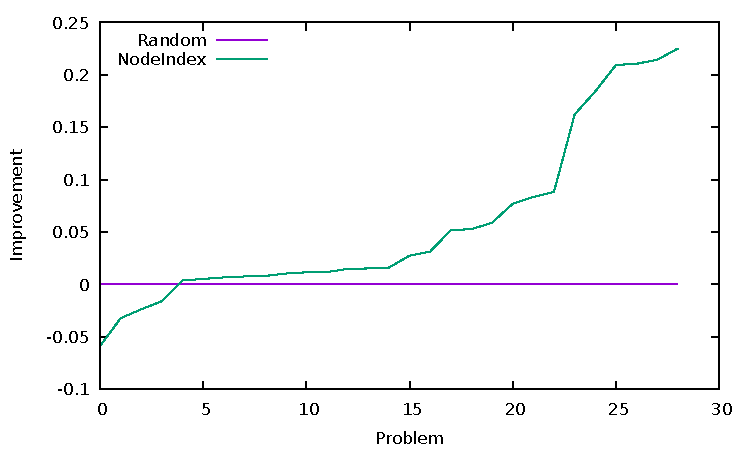
\includegraphics[scale=0.4]{Experiments/E1/imp/impro.pdf}
\end{figure}
\end{frame}

\begin{frame}
	\frametitle{Our improvements}
	\heading{Basic scheme}
    \begin{itemize}
    \item Step 1: Initialize Coloring (How to initialize coloring?)
    \item Step 2: Solve k-VCP (How to improve Tabucol?)
    \item Step 3: Reduce a color (How to reconstruct coloring?)
    \end{itemize}
\end{frame}
\begin{frame}
	\frametitle{Solving VCP by Tabucol}
    \framesubtitle{Step 1:How to initialize coloring?}
    	\begin{KITexampleblock}{     Our Node-index initialization vs Random initialization }
\begin{itemize}
\item
\textbf{Node-index initialization} is to use c: $v_i \rightarrow i$ as the initial solution. 
\item
\textbf{Random initialization} is to build a coloring randomly.
\end{itemize} 
\begin{figure}
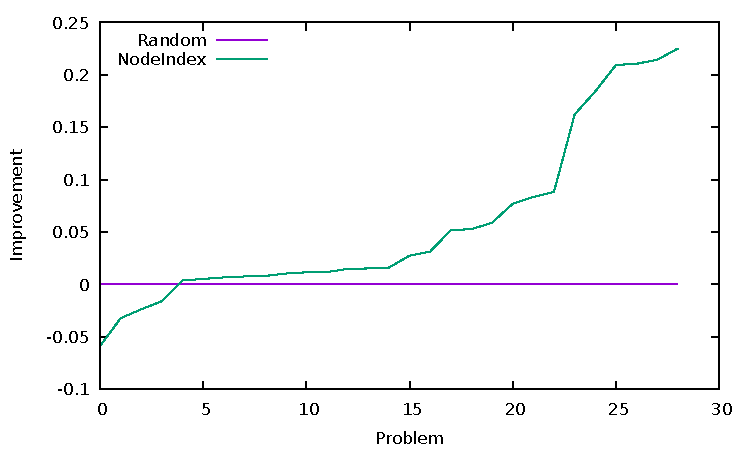
\includegraphics[scale=0.4]{Experiments/E1/imp/impro.pdf}
\end{figure}
\end{KITexampleblock}
\end{frame}
\begin{frame}
	\frametitle{Solving VCP by Tabucol}
    \framesubtitle{Step 2: How to improve Tabucol?}
    \begin{KITexampleblock}{ Our column-traverse vs row-traverse of solution matrix}
    \begin{itemize}
\item
To find next move, the maximum element in the solution matrix must be found. 
\item If more than one candidate exists, the first found one is chosen as the next step.
\item This matrix can be traversed row by row or column by column.  
    \end{itemize} 
 \begin{figure}
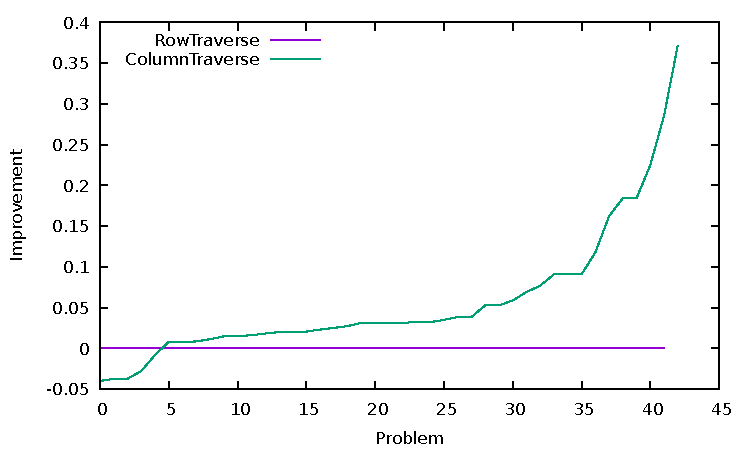
\includegraphics[scale=0.4]{Experiments/E3/imp/impro.pdf}
\end{figure}   
\end{KITexampleblock}
\end{frame}
\begin{frame}
	\frametitle{Solving VCP by Tabucol}
    \framesubtitle{Step 2: How to improve Tabucol?}
    \begin{KITexampleblock}{ Statistic matrix}
    \begin{itemize}
\item The Tabucol algorithm uses a tabu list to avoid short-term cycling.
\item To recognize long-term cycling, a \emph{statistic matrix S} is added. 
\item The $S_{ij}$ represents how many times a one-step move $[i,j]$ was chosen as the next step. 
\item The candidate with the smallest statistic value will be chosen in the next step.  
    \end{itemize} 
 \begin{figure}
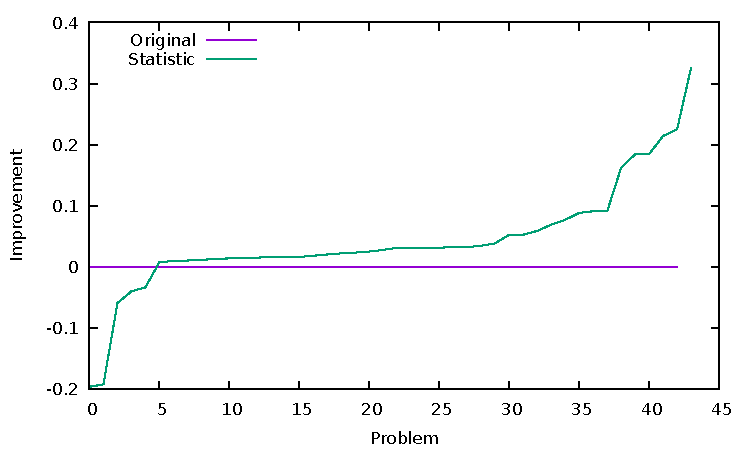
\includegraphics[scale=0.4]{Experiments/E4/imp/impro.pdf}
\end{figure}   
\end{KITexampleblock}
\end{frame}
\begin{frame}
	\frametitle{Solving VCP by Tabucol}
    \framesubtitle{Step 3: How to reconstruct new coloring?}
\begin{KITexampleblock}{An observation}
It seems that the solution loses its potential in the process of reducing colors iteratively. So it should be helpful to use a new and perhaps more potential coloring.
\end{KITexampleblock}
 \begin{KITexampleblock}{Replace by a randomly generated solution}
We replace the current illegal solution  occasionally by a new randomly generated coloring of the same size.
 \begin{figure}
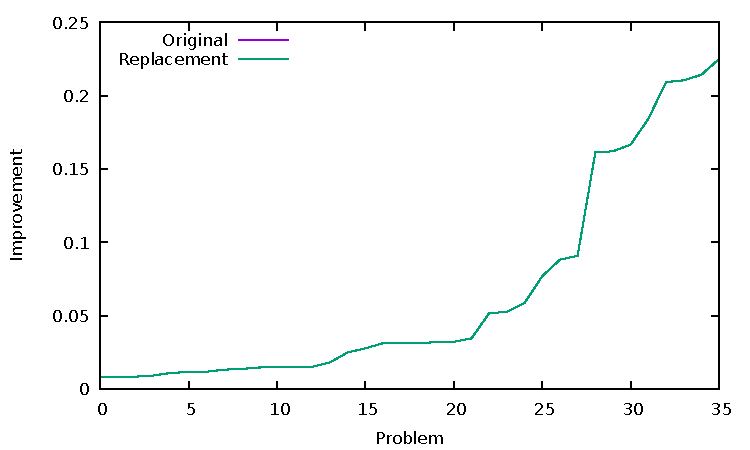
\includegraphics[scale=0.4]{Experiments/E2/imp/impro.pdf}
\end{figure}   
\end{KITexampleblock}
\end{frame}
\begin{frame}
  \frametitle{Outline}

\heading{The vertex coloring problem}
  \begin{itemize}
  \item k-VCP
  \item VCP
  \end{itemize}
\heading{{The Tabucol algorithm}}
\heading{Solving VCP by Tabucol}
  \begin{itemize}
  \item Basic scheme
  \item Our improvements
  \end{itemize}
\heading{\color<beamer:1>{red}{Our Parallel GCP-solver}}
  \begin{itemize}
  \item Parameter combinations
  \item Our approaches
  \end{itemize}
        \heading{Conclusion}
\end{frame}
\begin{frame}
	\frametitle{Our Parallel GCP-solver}
    \framesubtitle{Parameter combinations}
    \begin{itemize}
    \item Most graphs get better results with the our suggestions. 
\item Some graphs get better results with the original GCP-solver.
    \item The agents run with different combinations of the suggestions ($L$, $\alpha$, the search directions and whether a statistic matrix is introduced).
    \end{itemize}
\end{frame}
\begin{frame}
	\frametitle{Our Parallel GCP-solver}
    \framesubtitle{Parameter combinations}
    \small
      \begin{tabular}{| l | l l l l l l |p{2cm}|}
   \hline
Index&L& $\alpha$ &Initialization&Replace&Traverse& Statistic\\ \hline
1&9 &0.38 &Node-Index&true&Column&true\\
2&1 &0.77&Node-Index&true&Column&true\\
3&11 &0.90&Node-Index&true&Column&true \\
4&17 &0.59&Random&true&Column&true \\
5&18 &0.42&Node-Index&false&Column&false\\\hline
6&4 &0.92&Node-Index&true&Column&true \\
7&16 &0.76&Node-Index&false&Row&false\\
8&17 &0.47&Node-Index&false&Column&false\\
9&2 &0.60&Node-Index&true&Column&false\\
10&2 &0.54&Node-Index&false&Column&true\\\hline
11&5 &0.46&Random&true&Column&true\\
12&11 &0.63&Random&true &Column&true\\
13&7 &0.83&Node-Index&true&Column&true\\
14&8 &0.98&Node-Index&false &Row&true\\
15&18 &0.58&Node-Index&true&Column&false \\
16&13 &0.90&Node-Index&false&Column&true \\\hline
    \end{tabular}
\end{frame}
\begin{frame}
	\frametitle{Our Parallel GCP-solver}
    \framesubtitle{Parameter combinations}
    \small
      \begin{tabular}{| l | l l l l l l |p{2cm}|}
   \hline
Index&L& $\alpha$ &Initialization&Replace&Traverse& Statistic\\ \hline

17&20 &0.56&Node-Index&true &Column&false\\
18&10&0.95&Node-Index&true &Column&true\\
19&15 &0.55&Node-Index&true&Row&true\\
20&17 &0.39&Node-Index&true&Column&true \\\hline
21&18 &0.52&Node-Index&false&Column&true\\
22&11 &0.32&Node-Index&true&Column&true \\
23&15 &0.62&Node-Index&false&Column&true \\
24&6 &0.94&Random&true&Column&true\\
25&9 &0.94&Node-Index&false&Column &false\\\hline
26&12 &0.96&Node-Index&true&Column&true\\
27&16 &0.58&Node-Index&false&Column&true\\
28&9 &0.45&Node-Index&false&Column&true\\
29&19 &0.95&Node-Index&true&Column&true \\
30&18 &0.31&Node-Index&true&Column &false\\\hline
31&6 &0.50&Node-Index&false&Column&false\\
32&15 &0.93&Node-Index&false&Column &false\\\hline
    \end{tabular}
\end{frame}
\begin{frame}
	\frametitle{Our Parallel GCP-solver}
    \framesubtitle{1st Approach: The pure portfolio approach}
    \begin{itemize}
\item The agents run the GCP solver with different parameter combinations. 
\item After collecting the solutions found by each agent, the search takes the coloring of the minimum size as the result.
    \end{itemize}
\end{frame}
\begin{frame}
	\frametitle{Our Parallel GCP-solver}
    \framesubtitle{2nd Approach: Forced color reducing}
\begin{itemize}
\item This approach is based on the pure portfolio approach.
\item The agents share the minimum size.
\item One agent has already found a $k$-coloring and broadcasts it.
\item With this notification, all agents search for a legal $k-1$ coloring.
\end{itemize}
\begin{figure}
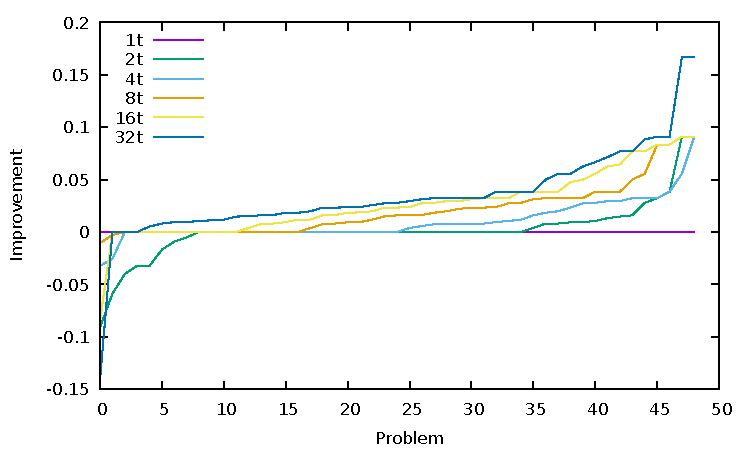
\includegraphics[scale=0.6]{Experiments/E6/imp/impro.pdf}
\end{figure}
\end{frame}

\begin{frame}
	\frametitle{Our Parallel GCP-solver}
    \framesubtitle{3rd Approach: Tabu sharing}
    \begin{itemize}
\item A tabu list records the search path to avoid short-term cycling.
\item The agents share the ``traps'' of local search loops. 
    \end{itemize}
 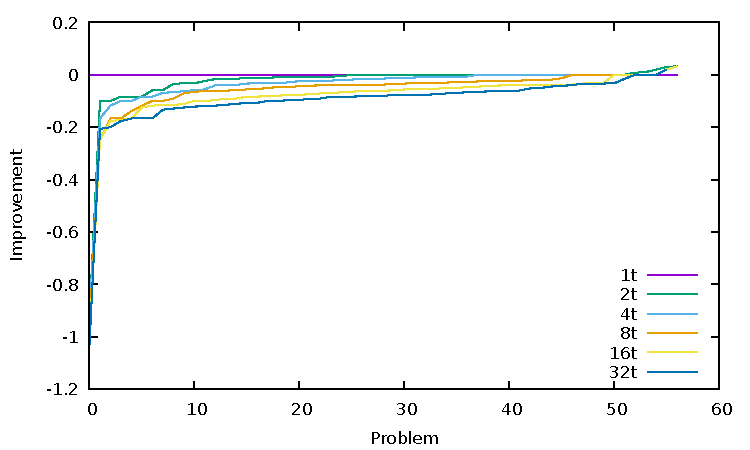
\includegraphics[scale=0.6]{Experiments/E7/imp/impro.pdf}
\end{frame}

\begin{frame}
	\frametitle{Our Parallel GCP-solver}
    \framesubtitle{4th Approach: Statistic sharing}
\begin{itemize}
\item To recognize long-term cycling, a \emph{statistic matrix S} is added. 
\item The $S_{ij}$ represents how many times a one-step move $[v_i,j]$ was chosen as the next step. 
\item The candidate with the smallest statistic value will be chosen in the next step.  
\item The agents use one common statistic matrix.\\
  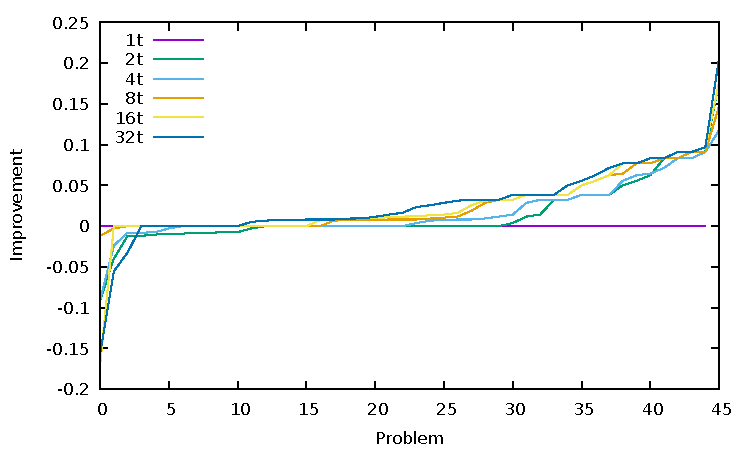
\includegraphics[scale = 0.6]{Experiments/E8/imp/impro.pdf}
\end{itemize}
\end{frame}
\begin{frame}
  \frametitle{Outline}

\heading{The vertex coloring problem}
  \begin{itemize}
  \item k-VCP
  \item VCP
  \end{itemize}
  
\heading{The Tabucol algorithm}
\heading{Solving VCP by Tabucol}
  \begin{itemize}
  \item Basic scheme
  \item Our improvements
  \end{itemize}
\heading{Our Parallel GCP-solver}
  \begin{itemize}
  \item Parameter combinations
  \item Our approaches
  \end{itemize}
\heading{ \color<beamer:1>{red}Conclusion} 
\end{frame}
\begin{frame}
	\frametitle{Conclusion}
\heading{Our improvement:}
\begin{itemize}
\item An algorithm solves the VCP with parallel Tabucol searches.
\item The statistic matrix recognizes long-term cycling and brings improvement to our algorithm.
\item Certain information exchange (minimum size, statistic matrix) can improve the performance of the parallel search. 
\end{itemize}

\heading{Comparison of our GCP-solver with DSATUR, PASS, TRICK:} 
\begin{itemize}
\item  50 of 68 (73\%) benchmark graphs get best results with our solver.
\item  20 of 68 (29\%) benchmark graphs get unique best results with our solver.
\end{itemize}
\heading{Further work}
\begin{itemize}
\item Using different  search strategies
\item Using different cooperation strategies
\item Using different algorithms in agents
\end{itemize}
\end{frame}
\begin{frame}

 \begin{figure}

\includegraphics[scale=0.2]{1/thank-you-for-your-attention-any-questions-78.png}
\end{figure}   
\end{frame}
\end{document}
